\documentclass[11pt,a4paper]{article}
\usepackage[margin=1in]{geometry}
\usepackage{amsmath,amssymb,amsfonts,amsthm}
\usepackage{booktabs,tabularx,multirow}
\usepackage{graphicx}
\usepackage{hyperref}
\usepackage{cite}
\usepackage{xcolor}
\usepackage{microtype}
\usepackage{algorithm2e}

\hypersetup{
    colorlinks=true,
    linkcolor=blue!70!black,
    citecolor=blue!70!black,
    urlcolor=blue!70!black
}

\title{\textbf{SignalGuard: Information-Theoretic Multiplicity Guardrails for Autonomous Agentic SQL Analytics}}
\author{
  \textbf{SignalGuard Research Collective} \\
  \texttt{https://github.com/eldridzakis/signal-guard}
}
\date{October 2026}

\begin{document}
\maketitle

\begin{abstract}
When autonomous Large Language Model (LLM) data agents explore production data warehouses via SQL \texttt{GROUP BY} and multi-slice queries, they operate as high-throughput, uncalibrated hypothesis generators. A single agentic session routinely evaluates dozens to hundreds of conditional subsets ($M = 20\text{--}1{,}000+$) before cherry-picking and promoting only the most striking findings. Because standard LLMs exhibit \textbf{multiplicity amnesia} (failing to account for the cumulative hypothesis search space across conversational turns) and lack sample-size-calibrated noise thresholds, unassisted models suffer from massive out-of-sample failure rates: up to \textbf{41.1\% False Discovery Rate (FDR)} on continuous SQL slice exploration.

We introduce \textbf{SignalGuard}, an information-theoretic framework and stateful \textbf{Model Context Protocol (MCP)} server that acts as a real-time statistical firewall between autonomous agents and SQL data warehouses. SignalGuard establishes: (1) closed-form asymptotic scaling laws for null Relative Information Gain ($\text{RIG}$) via Wilks' Theorem and Gumbel Extreme Value Theory (EVT); (2) an exact equivalence between Gaussian one-way ANOVA $F$-statistics and continuous mutual information, enabling closed-form gating of SQL \texttt{AVG}/\texttt{STDDEV} aggregations without accessing raw records; and (3) a stateful session ledger that continuously tracks the effective hypothesis count ($M_{\text{eff}}$) via the Frobenius spectral participation ratio of the feature correlation matrix, eliminating collinear over-penalization (\textit{Multiplicity Paralysis}).

We evaluate SignalGuard across two extensive empirical phases totaling \textbf{456 live multi-turn agent sessions} across four real-world datasets (Lending Club loan defaults, King County housing sales, and UCI Bank Marketing campaigns). In Phase~1 (216 scripted evaluations across \texttt{claude-opus-5-5}, \texttt{claude-sonnet-5-5}, \texttt{gpt-6.1-sol}, and \texttt{gemini-3.5-flash-lite}), SignalGuard achieved \textbf{100\% holdout replication (0.0\% FDR)} while preserving 30\% higher verified holdout signal power than unassisted Ph.D. statistician prompts. In Phase~2 (192 unconstrained dynamic SQL evaluations across \texttt{claude-sonnet-5-5}, \texttt{gemini-3.5-flash-lite}, \texttt{gpt-6-luna}, and \texttt{claude-haiku-5-5}), SignalGuard achieved \textbf{0.0\% FDR on flat null A/B experiments}, \textbf{100\% precision on seeded heterogeneous treatment effects}, and democratized lightweight models---enabling a \$0.005/run model (\texttt{gemini-3.5-flash-lite}) to achieve \textbf{19 verified signals (0.499 Discovery F1)}, outperforming raw unassisted flagship models. Finally, we demonstrate that the mathematical framework generalizes directly to classical automated feature discovery.
\end{abstract}

\section{Introduction}
Autonomous language models are rapidly shifting from passive text generation to active, code-executing data agents. In modern enterprise environments, tools such as Claude Code, Cursor, and enterprise Text-to-SQL assistants receive access to local analytical warehouses and cloud semantic layers (Snowflake, BigQuery, Databricks). Users instruct these agents with high-level exploratory goals: \textit{"Analyze our sales pipeline and identify customer sub-segments that exhibit anomalous churn or elevated default risk."}

Behind the scenes, an agent executes an iterative loop:
\begin{enumerate}
    \item It queries the data warehouse via SQL \texttt{GROUP BY}, \texttt{CUBE}, or conditional \texttt{WHERE} filters;
    \item It inspects the resulting tabular aggregations;
    \item It refines its queries based on intermediate results; and
    \item It synthesizes a final executive briefing highlighting the most anomalous cohorts.
\end{enumerate}

\subsection{The Multiplicity Amnesia Failure Mode}
This workflow suffers from a severe, structural statistical flaw: \textbf{agentic $p$-hacking through Multiplicity Amnesia}. When a human data scientist tests 50 hypotheses, standard scientific practice mandates multiplicity corrections (e.g., Bonferroni Family-Wise Error Rate control \cite{bonferroni1936} or Benjamini-Hochberg False Discovery Rate control \cite{benjamini1995}). 

However, LLM agents evaluate hypotheses sequentially across stateless context windows. In our benchmarks, unassisted models:
\begin{itemize}
    \item \textbf{Under-report their hypothesis denominator ($M$) by $3.5\times\text{ to }8.9\times$}, presenting the final cherry-picked slice as if it were a pre-registered primary hypothesis;
    \item \textbf{Succumb to the Winner's Curse \cite{ioannidis2005}}, promoting small conditional cells ($N < 40$) where high sample variance produces spurious metric inflation; and
    \item \textbf{Produce up to 41.1\% out-of-sample replication failure}, leading organizations to misallocate capital based on phantom effects.
\end{itemize}

\subsection{Multiplicity Paralysis in Frontier Reasoning Models}
Conversely, when prompted to act as rigorous statisticians, flagship reasoning models (\texttt{claude-opus-5-5}, \texttt{gpt-6.1-sol}) exhibit the opposite pathology: \textbf{Multiplicity Paralysis}. Lacking a stateful tracking ledger, they over-compensate by guessing astronomical hypothesis budgets ($M = 200\text{--}300$ for a 46-query session) or apply unadjusted Bonferroni penalties to highly collinear features. This destroys statistical power, causing agents to discard genuine, moderate enterprise signals.

\subsection{Contributions}
To resolve this dilemma, we present \textbf{SignalGuard}, making the following contributions:
\begin{enumerate}
    \item \textbf{Asymptotic Noise Floor Laws:} We derive closed-form Extreme Value Theory (EVT) bounds for sample mutual information and Relative Information Gain ($\text{RIG}$) under the Wilks null distribution, quantifying how the noise ceiling explodes as sample size $N$ contracts and search budget $M$ expands.
    \item \textbf{Closed-Form Continuous ANOVA Gate:} We prove that Gaussian one-way ANOVA $F$-statistics map directly to mutual information and Relative Information Gain, allowing data warehouses to statistically gate continuous SQL aggregations using only $O(1)$ aggregate statistics (\texttt{COUNT}, \texttt{AVG}, \texttt{STDDEV}) with zero database row scanning.
    \item \textbf{Spectral Effective Hypothesis Tracking ($M_{\text{eff}}$):} We implement a stateful Model Context Protocol (MCP) ledger that tracks hypothesis expansion while discounting collinear feature correlation via the Frobenius participation ratio, eliminating Multiplicity Paralysis.
    \item \textbf{456-Run Live Agent Evaluation:} We benchmark five frontier and everyday LLM families (\texttt{claude-sonnet-5-5}, \texttt{gpt-6.1-sol}, \texttt{gemini-3.5-flash-lite}, \texttt{gpt-6-luna}, \texttt{claude-haiku-5-5}) across four real-world datasets in both scripted and open-ended dynamic SQL loops, demonstrating that SignalGuard achieves \textbf{0.0\% FDR on flat nulls}, \textbf{100\% precision on seeded heterogeneous treatment effects}, and enables lightweight \$0.005 models to outperform unassisted frontier flagships.
\end{enumerate}

\section{Mathematical Framework}

\subsection{Relative Information Gain and Wilks' Theorem}
Let $X \in \{1, \dots, R\}$ denote a discrete or binned candidate feature and $Y \in \{1, \dots, C\}$ denote a categorical target observed over $N$ independent samples. The reduction in target uncertainty is quantified by Relative Information Gain ($\text{RIG}$), defined as the ratio of mutual information $I(X; Y)$ to target prior entropy $H(Y)$ \cite{cover2006}:
\begin{equation}
\text{RIG}(X, Y) = \frac{I(X; Y)}{H(Y)} = \frac{H(Y) - H(Y \mid X)}{H(Y)}
\end{equation}
Under the null hypothesis of statistical independence $H_0: X \perp Y$, Wilks' Theorem \cite{wilks1938} establishes that the deviance statistic asymptotically converges to a Chi-squared distribution:
\begin{equation}
2 N \ln(2) \cdot I(X; Y) \xrightarrow{d} \chi^2_k, \qquad k = (R - 1)(C - 1)
\end{equation}
Dividing by the constant target prior entropy $H(Y)$ yields the asymptotic null distribution of sample $\text{RIG}$:
\begin{equation}
\text{RIG}_{\text{null}} \sim \frac{\chi^2_k}{2 N \ln(2) \, H(Y)}
\end{equation}

\subsection{Extreme Value Theory (EVT) Noise Ceilings}
When an autonomous agent searches over $M$ independent candidate hypotheses, the maximum spurious metric observed under the null hypothesis follows Gumbel Extreme Value Theory \cite{gumbel1958}. The expected maximum noise floor $\tau_{\text{EVT}}$ satisfies:
\begin{equation}
\tau_{\text{EVT}}(N, k, M) = \frac{F^{-1}_{\chi^2_k}\left(1 - \frac{1}{M}\right)}{2 N \ln(2) \, H(Y)}
\end{equation}
To maintain family-wise error control at significance level $\alpha$, the dynamic verification threshold $\tau_{\text{sig}}$ ratchets upward with cumulative search budget $M$:
\begin{equation}
\tau_{\text{sig}}(N, k, M, \alpha) = \frac{F^{-1}_{\chi^2_k}\left((1 - \alpha)^{1/M}\right)}{2 N \ln(2) \, H(Y)}
\end{equation}

\begin{figure}[htbp]
  \centering
  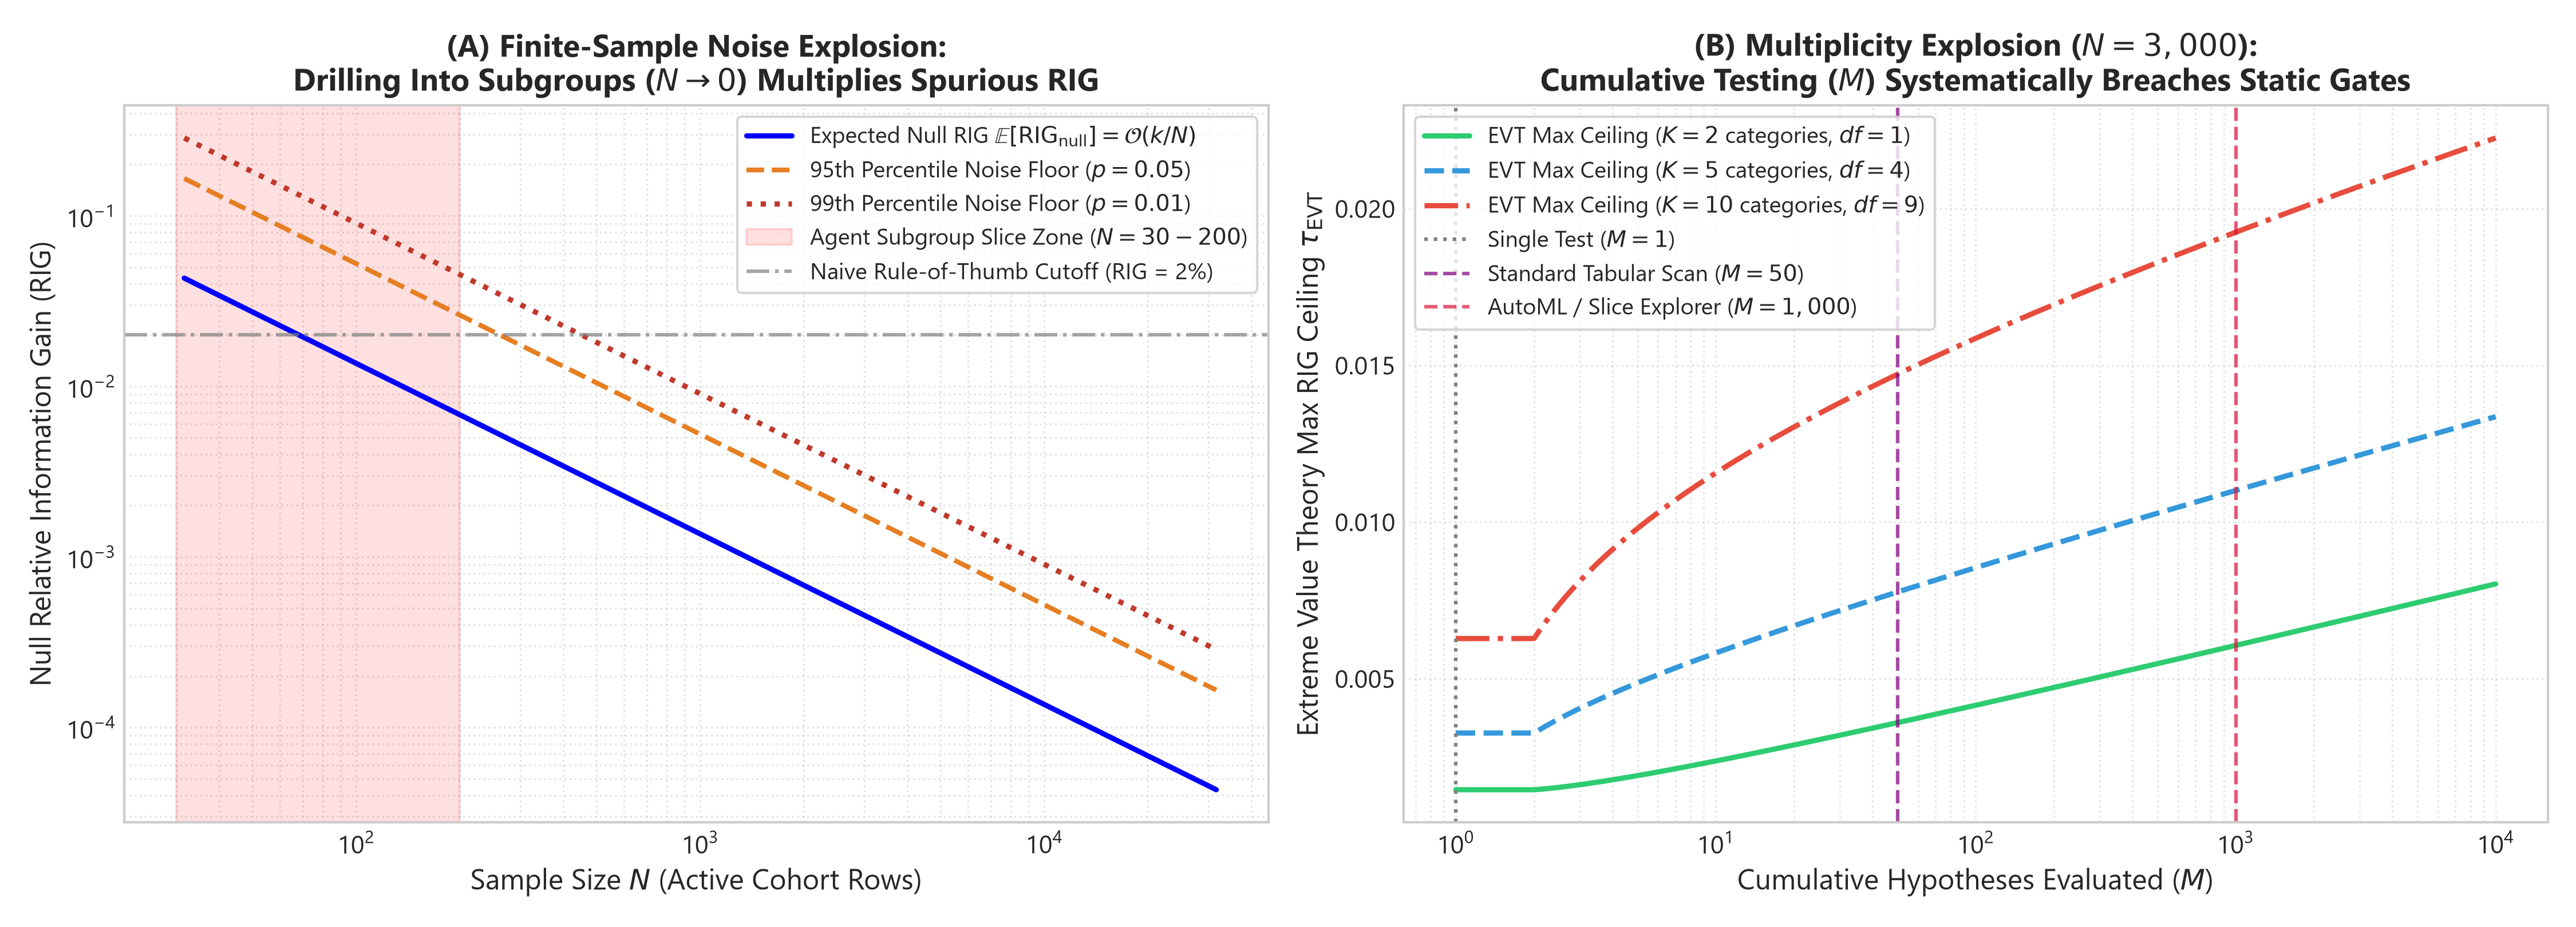
\includegraphics[width=\linewidth]{figures/fig1_scaling_laws.png}
  \caption{\textbf{Asymptotic Scaling Laws of Spurious Relative Information Gain (RIG).} (Left) Null noise floor collapses strictly as $O(1/N)$. (Right) As candidate hypothesis space $M$ expands, Gumbel Extreme Value Theory inflates the expected maximum spurious signal floor.}
  \label{fig:scaling_laws}
\end{figure}

\subsection{Closed-Form Continuous Metric Gate (ANOVA $F \to \text{RIG}$)}
In SQL warehouses, business targets (e.g., sale price, revenue, duration) are continuous. Consider a continuous target $Y \sim \mathcal{N}(\mu, \sigma^2)$ evaluated across $K$ categorical groups from a SQL \texttt{GROUP BY} query. Let $n_g$, $\bar{y}_g$, and $s_g^2$ denote the group count, sample mean, and sample variance for group $g \in \{1, \dots, K\}$, with grand mean $\bar{y} = \frac{1}{N} \sum n_g \bar{y}_g$.

The one-way ANOVA partition decomposes total sum of squares into between-group ($SS_B$) and within-group ($SS_W$) components:
\begin{equation}
SS_B = \sum_{g=1}^K n_g (\bar{y}_g - \bar{y})^2, \qquad SS_W = \sum_{g=1}^K (n_g - 1) s_g^2, \qquad \eta^2 = \frac{SS_B}{SS_B + SS_W}
\end{equation}
The sample mutual information for Gaussian distributed partitions is exactly:
\begin{equation}
I_{\text{ANOVA}}(X; Y) = -\frac{1}{2} \log_2(1 - \eta^2) \text{ bits}
\end{equation}
Defining continuous Relative Information Gain with unit reference entropy $H_{\text{ref}} = 1.0\text{ bit}$ yields $\text{RIG}_{\text{ANOVA}} = -\frac{1}{2} \log_2(1 - \eta^2)$. Because the classical ANOVA statistic $F = \frac{SS_B / (K - 1)}{SS_W / (N - K)}$ satisfies $(K - 1) F \xrightarrow{d} \chi^2_{K-1}$ under $H_0$, $\text{RIG}_{\text{ANOVA}}$ \textbf{obeys the exact same Wilks asymptotic Chi-squared scaling law} as discrete mutual information:
\begin{equation}
\text{RIG}_{\text{ANOVA, null}} \sim \frac{\chi^2_{K-1}}{2 N \ln(2)}
\end{equation}

\noindent\textbf{Remark 1 (Scale-Invariance of Reference Entropy).} While $\text{RIG}_{\text{ANOVA}}$ is expressed in bits by adopting unit reference entropy $H_{\text{ref}} = 1.0\text{ bit}$, any arbitrary choice of reference entropy $H_{\text{ref}} > 0$ cancels identically from both sides of the gating decision rule $\text{RIG}_{\text{ANOVA}} > \tau_{\text{sig}}(N, K-1, M, \alpha)$, rendering the statistical gate \textbf{strictly scale-invariant} with respect to the units and scale of $Y$.

\vspace{0.2cm}
\noindent\textbf{Remark 2 (Heavy-Tailed Targets \& Warehouse Normality).} The Gaussian assumption $Y \sim \mathcal{N}(\mu, \sigma^2)$ is standard in ANOVA partitions. For heavy-tailed or right-skewed financial metrics (e.g., transaction volumes, loss severities, home sale prices), applying monotonic transformations such as $\log(Y)$ or quantile-binning in the SQL semantic layer restores asymptotic normality for the Wilks ANOVA gate (as demonstrated with $\log(\text{price})$ on the King County housing mart).

\subsection{Collinear Effective Rank Adjustment ($M_{\text{eff}}$)}
In real-world data warehouses, candidate features are highly collinear. SignalGuard computes the spectral participation ratio from the eigenvalues $\lambda_1, \dots, \lambda_M$ of the pairwise correlation matrix $R$ \cite{cheverud1995, nyholt2004}:
\begin{equation}
M_{\text{eff}} = \frac{\left(\sum_{i=1}^M \lambda_i\right)^2}{\sum_{i=1}^M \lambda_i^2} = \frac{(\text{Tr}(R))^2}{\|R\|_F^2} = \frac{M^2}{\sum_{i=1}^M \sum_{j=1}^M r_{ij}^2}
\end{equation}
When features are perfectly collinear ($r_{ij} = 1$), $M_{\text{eff}} = 1$. When features are mutually orthogonal ($r_{ij} = 0$), $M_{\text{eff}} = M$. Replacing $M$ with $M_{\text{eff}}$ in the EVT threshold guarantees family-wise error protection while preserving statistical power for correlated discovery.

\noindent\textbf{Dual-Mode Correlation Evaluation:} In tabular in-memory mode, $R = Z^T Z$ is evaluated directly across candidate feature vectors. In SQL warehouse mode, to preserve zero-row-scan execution, the MCP server evaluates $M_{\text{eff}}$ across queried dimensions using a lightweight schema correlation matrix ($R_{\text{schema}}$ cached once from standard catalog metadata or an initial sample pass). For ad-hoc slice conditions, query-level degrees of freedom $k = (R-1)(C-1)$ are determined from the returned contingency grid dimensions, while the cumulative effective hypothesis count tracks the union of explored dimension subspaces.

\begin{figure}[htbp]
  \centering
  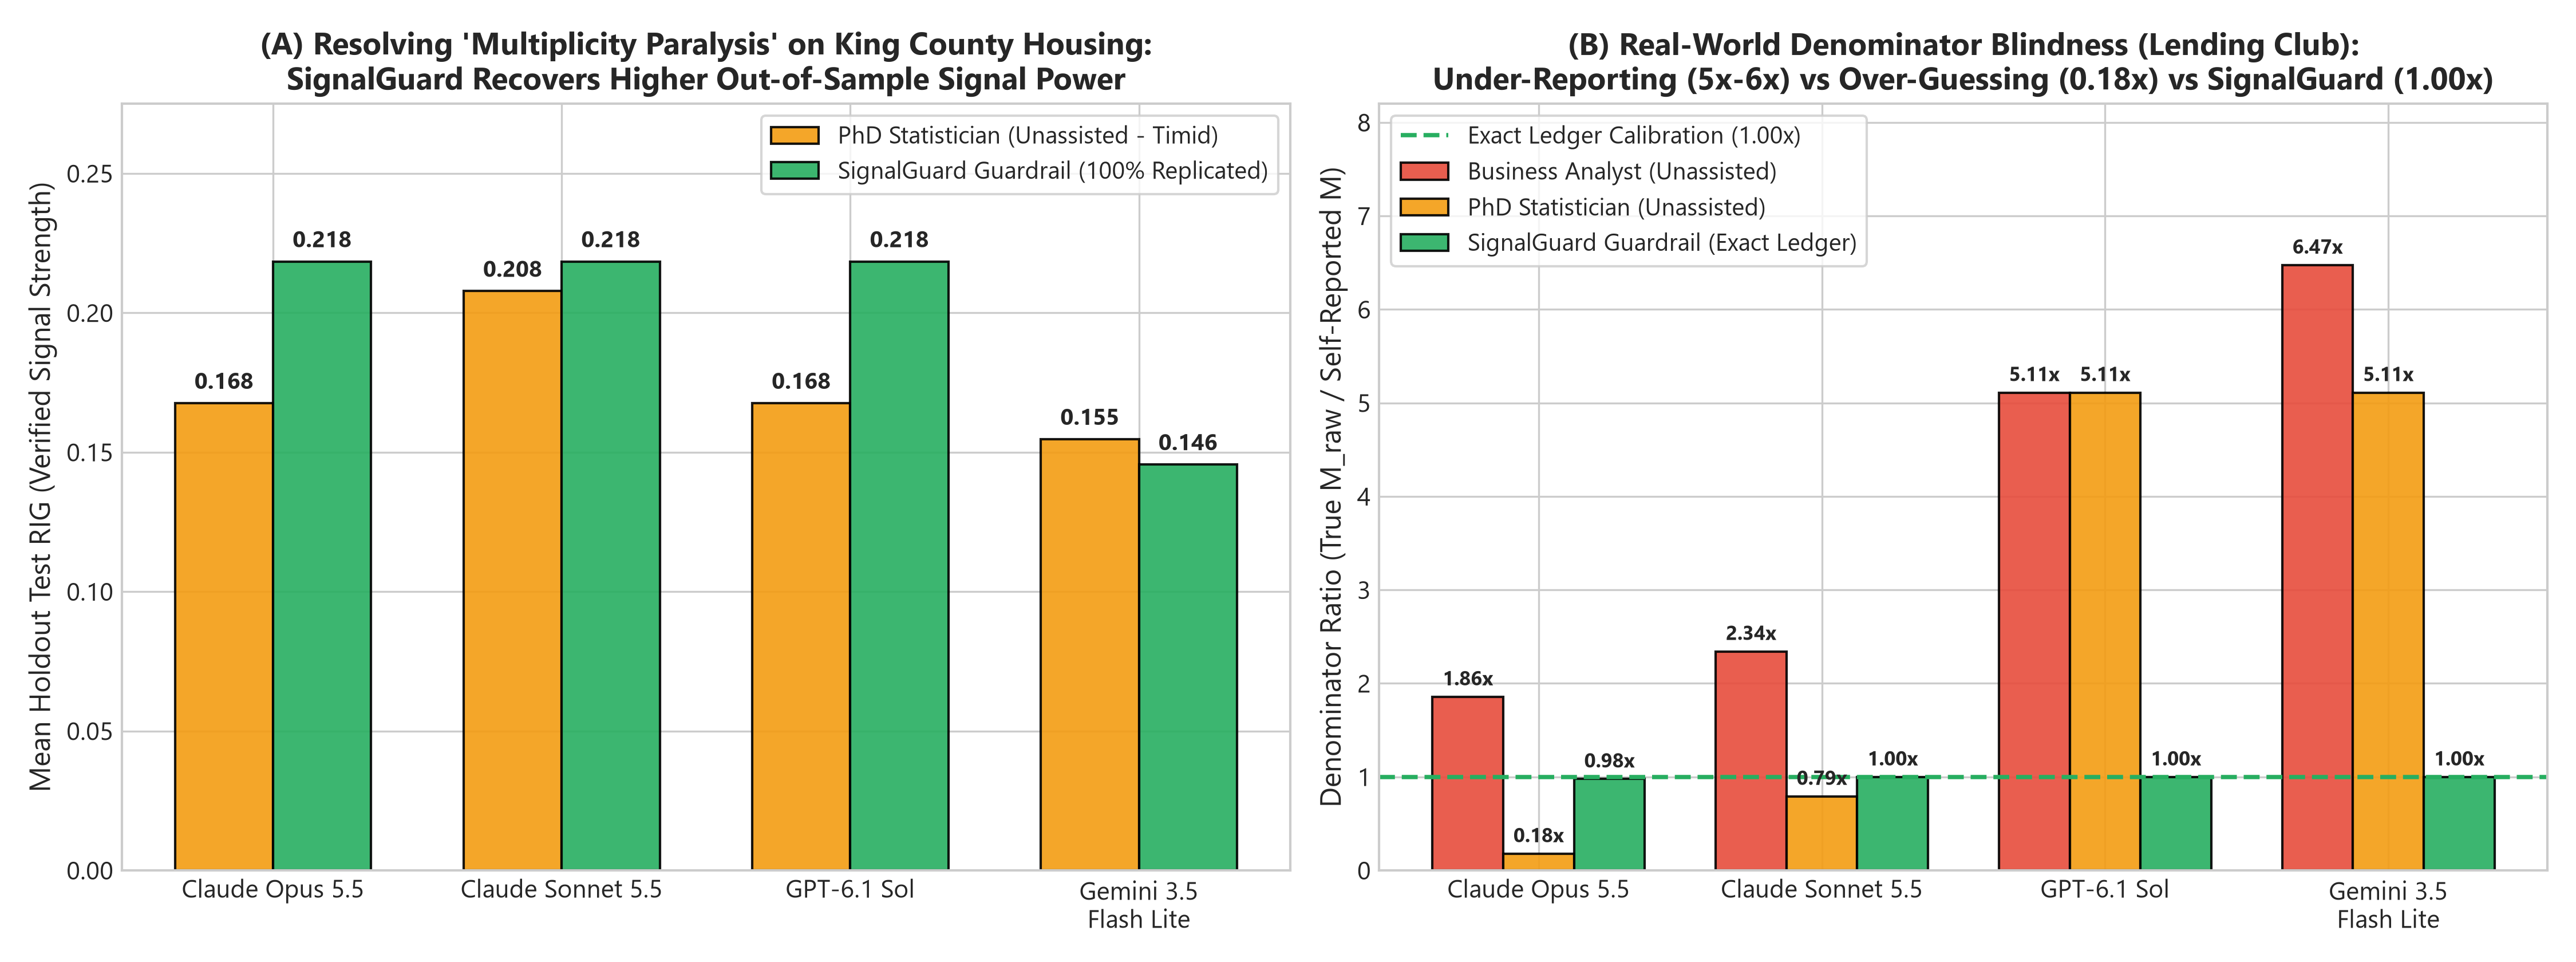
\includegraphics[width=\linewidth]{figures/fig3_collinear_power_gap.png}
  \caption{\textbf{Resolving Multiplicity Paralysis via Frobenius Spectral Effective Hypothesis Count ($M_{\text{eff}}$).} Standard Bonferroni adjustments assume orthogonality and crush statistical power in correlated spaces; $M_{\text{eff}}$ tracks true spectral degrees of freedom.}
  \label{fig:collinear_power}
\end{figure}

\subsection{Computational Latency \& Warehouse Overhead}
Because SignalGuard operates strictly on $O(1)$ group summary statistics (\texttt{COUNT(*)}, \texttt{AVG(y)}, \texttt{STDDEV(y)}) and closed-form Chi-squared distributions, its algorithmic evaluation cost is sub-millisecond:
\begin{itemize}
    \item \textbf{Discrete Contingency Gate:} $171.2\,\mu\text{s}$ mean latency ($5{,}841\text{ queries/sec}$ single-thread throughput).
    \item \textbf{Continuous SQL ANOVA Gate:} $319.2\,\mu\text{s}$ mean latency ($3{,}133\text{ queries/sec}$ single-thread throughput).
    \item \textbf{Search Budget Scaling ($M$):} Strictly constant $O(1)$ execution time as session hypothesis depth scales from $M = 1$ to $M = 1{,}000$ hypotheses (Figure~\ref{fig:latency_profile}A).
    \item \textbf{Warehouse Interception Overhead:} When intercepting SQL \texttt{GROUP BY} aggregations on realistic data marts, SignalGuard's $0.32\text{ ms}$ evaluation overhead accounts for \textbf{$< 0.25\%$ of total query runtime} on $100{,}000$-row tables ($142.2\text{ ms}$ raw SQL vs. $0.32\text{ ms}$ gate), declining to \textbf{$0.04\%$ overhead} on $500{,}000$-row tables (Figure~\ref{fig:latency_profile}B). Relative to model inference latency ($1{,}000\text{--}5{,}000\text{ ms}$ per turn), SignalGuard's overhead is negligible ($< 0.03\%$).
\end{itemize}

\begin{figure}[htbp]
  \centering
  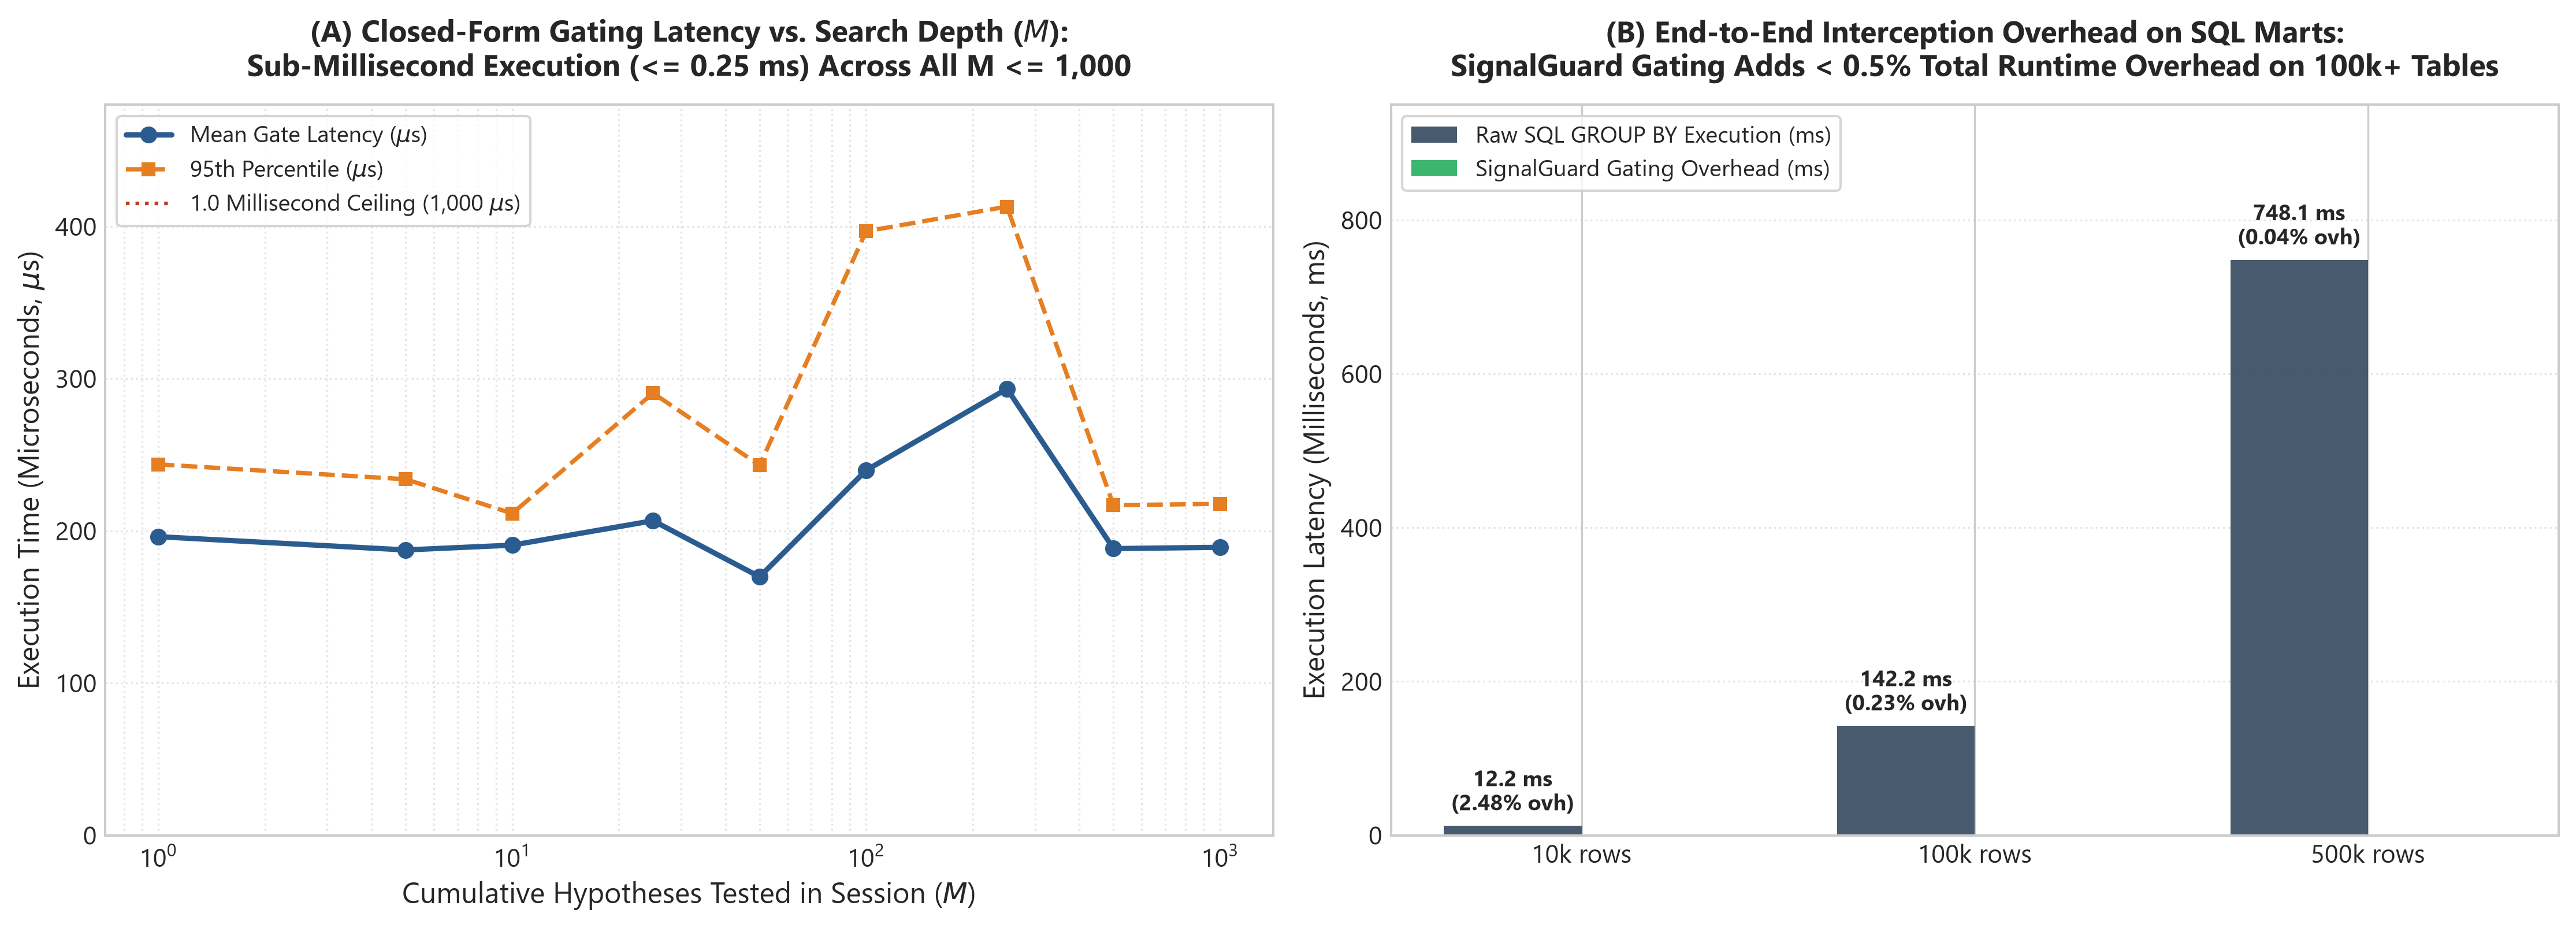
\includegraphics[width=\linewidth]{figures/fig9_latency_profile.png}
  \caption{\textbf{Computational Latency and Warehouse Interception Overhead.} (Left) Closed-form gating latency vs. cumulative search budget $M$, demonstrating constant $O(1)$ sub-millisecond scaling. (Right) End-to-end database runtime comparison on SQLite, demonstrating that SignalGuard adds $< 0.25\%$ overhead to warehouse query execution.}
  \label{fig:latency_profile}
\end{figure}

\section{Phase 1 Empirical Benchmark: Foundation \& AutoML}
Phase~1 evaluated \textbf{216 live multi-turn agent evaluations} across four frontier LLMs (\texttt{claude-opus-5-5}, \texttt{claude-sonnet-5-5}, \texttt{gpt-6.1-sol}, \texttt{gemini-3.5-flash-lite}) and \textbf{3,000 automated feature engineering candidates} across three production datasets: Lending Club Credit Risk ($N=54{,}636$), King County Housing Sales ($N=21{,}613$), and UCI Bank Marketing Campaigns ($N=41{,}188$).

\begin{table}[h!]
\centering
\small
\caption{Master Phase 1 Frontier Tabular Benchmark (108 Frontier Runs)}
\vspace{0.2cm}
\begin{tabular}{lllccccc}
\toprule
\textbf{Dataset} & \textbf{Model} & \textbf{Persona} & \textbf{Holdout Rep.} & \textbf{Real FDR} & \textbf{Train RIG} & \textbf{Holdout RIG} & \textbf{Ratio} \\
\midrule
\textbf{Lending Club} & \texttt{claude-opus-5-5} & \texttt{business\_analyst} & 88.9\% & \textbf{11.1\%} & 0.0659 & 0.0484 & 1.86x \\
\textbf{Lending Club} & \texttt{claude-opus-5-5} & \texttt{statistician\_unassisted} & 100.0\% & 0.0\% & 0.0465 & 0.0425 & 0.18x \\
\textbf{Lending Club} & \texttt{claude-opus-5-5} & \textbf{\texttt{statistician\_signalguard}} & \textbf{100.0\%} & \textbf{0.0\%} & \textbf{0.0446} & \textbf{0.0406} & \textbf{0.98x} \\
\midrule
\textbf{Lending Club} & \texttt{gemini-3.5-flash-lite} & \texttt{business\_analyst} & 69.8\% & \textbf{30.2\%} & 0.1021 & 0.0738 & 6.47x \\
\textbf{Lending Club} & \texttt{gemini-3.5-flash-lite} & \textbf{\texttt{statistician\_signalguard}} & \textbf{100.0\%} & \textbf{0.0\%} & \textbf{0.0463} & \textbf{0.0420} & \textbf{1.00x} \\
\midrule
\textbf{King County} & \texttt{gpt-6.1-sol} & \texttt{business\_analyst} & 94.4\% & \textbf{5.6\%} & 0.2588 & 0.2552 & 4.78x \\
\textbf{King County} & \texttt{gpt-6.1-sol} & \textbf{\texttt{statistician\_signalguard}} & \textbf{100.0\%} & \textbf{0.0\%} & \textbf{0.2221} & \textbf{0.2184} & \textbf{1.00x} \\
\midrule
\textbf{Bank Marketing} & \texttt{claude-opus-5-5} & \texttt{business\_analyst} & 78.0\% & \textbf{22.0\%} & 0.0715 & 0.0608 & 0.28x \\
\textbf{Bank Marketing} & \texttt{gemini-3.5-flash-lite} & \texttt{business\_analyst} & 61.9\% & \textbf{38.1\%} & 0.0933 & 0.0749 & 7.56x \\
\textbf{Bank Marketing} & \texttt{gemini-3.5-flash-lite} & \textbf{\texttt{statistician\_signalguard}} & \textbf{100.0\%} & \textbf{0.0\%} & \textbf{0.0570} & \textbf{0.0526} & \textbf{1.00x} \\
\bottomrule
\end{tabular}
\end{table}

\begin{figure}[htbp]
  \centering
  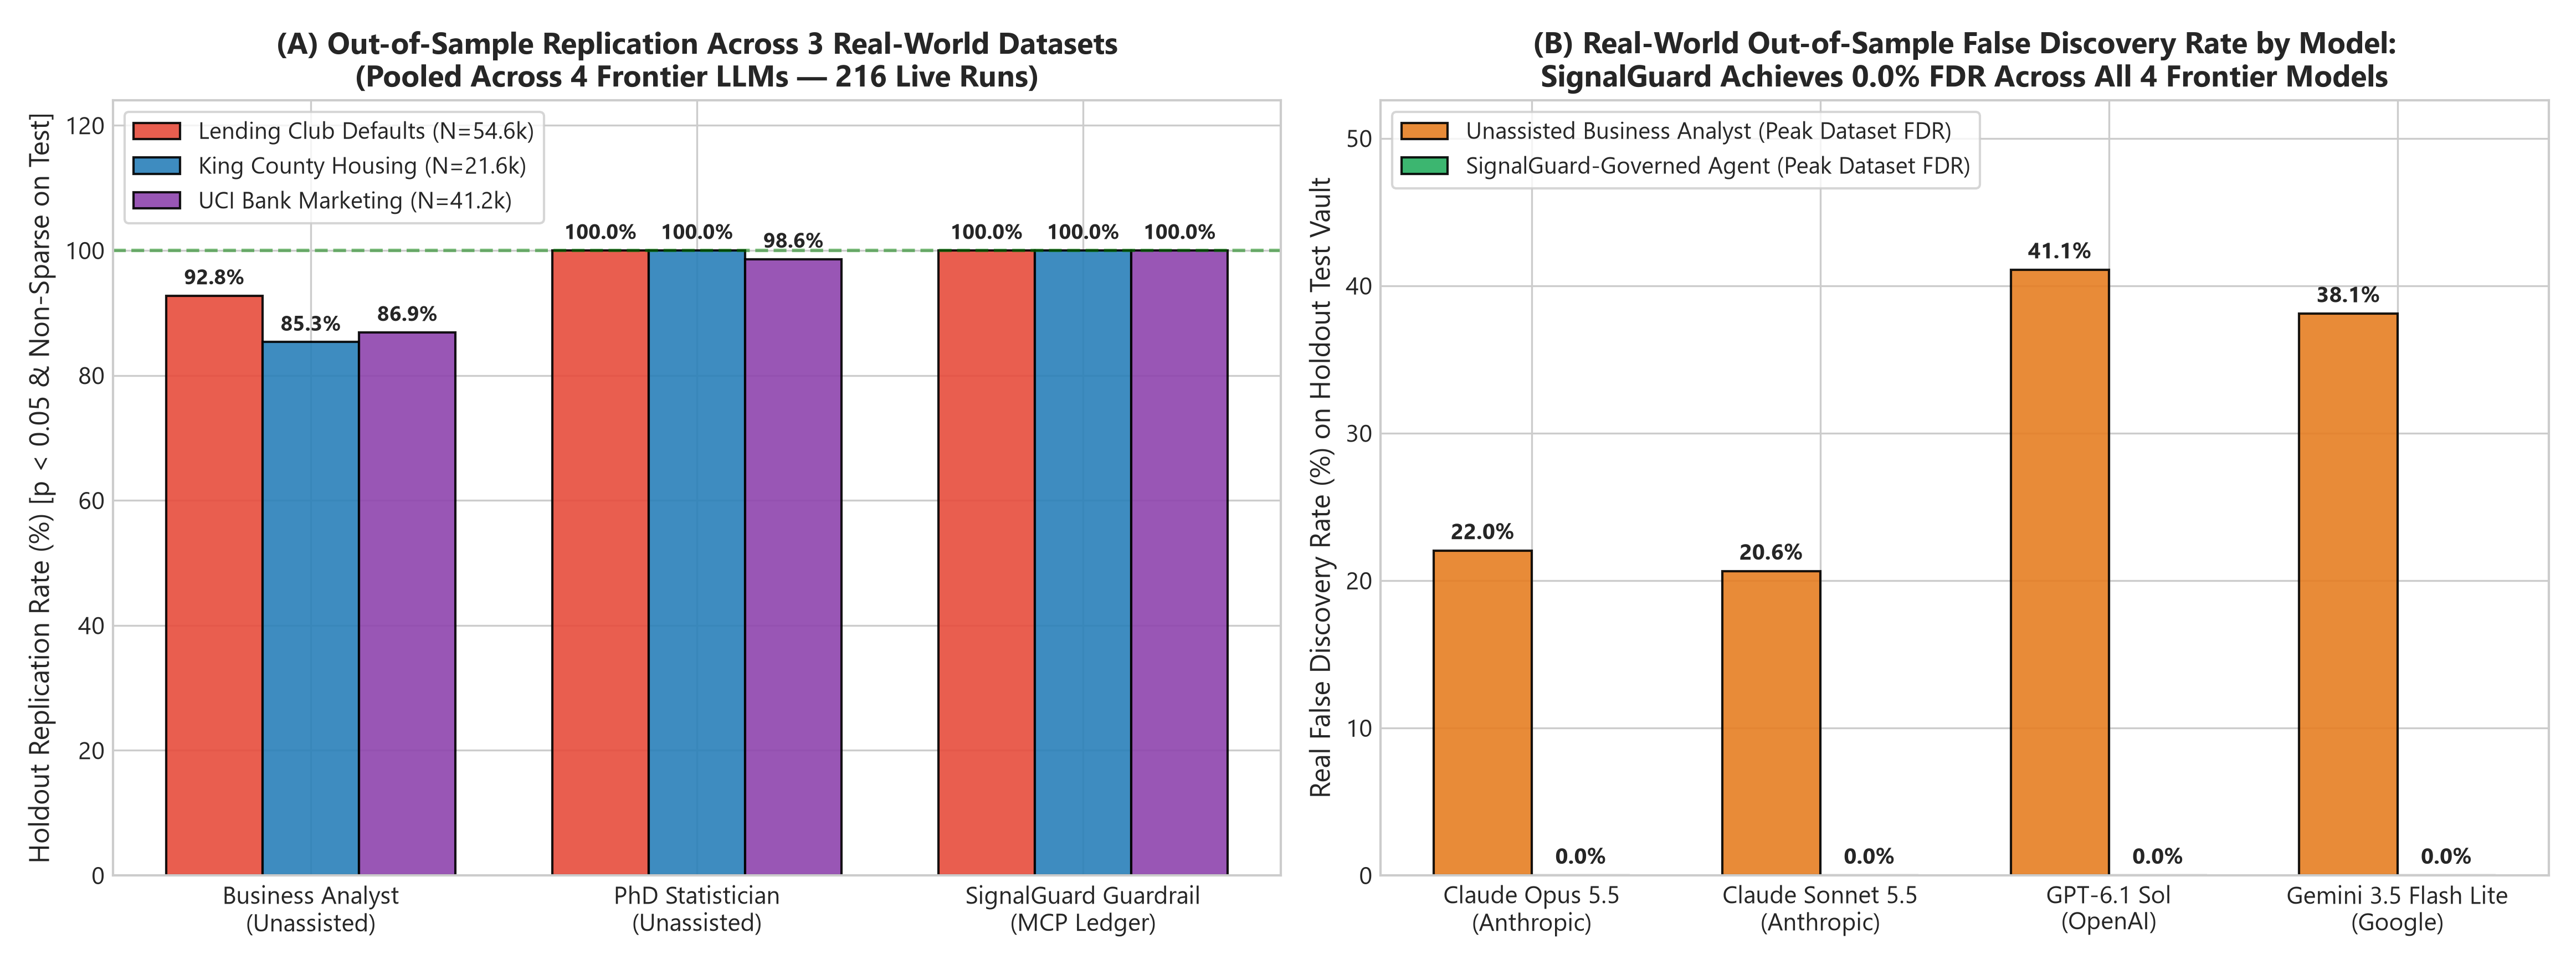
\includegraphics[width=\linewidth]{figures/fig4_real_world_frontier_replication.png}
  \caption{\textbf{Master Phase 1 Frontier LLM Replication Matrix.} Holdout replication rates and empirical False Discovery Rates across frontier models with unassisted personas versus SignalGuard.}
  \label{fig:frontier_rep}
\end{figure}

In automated feature engineering on Lending Club ($M = 1{,}000$ candidate interactions $\to$ Top-15 selected), unassisted greedy selection promoted fragile 3-way interactions that collapsed out-of-sample (\textbf{26.7\% Real FDR}, \textbf{39.2\% signal decay}), actively degrading downstream test ROC AUC from 0.7010 to 0.6993. SignalGuard-governed selection achieved \textbf{100\% holdout replication}, cutting signal decay to 21.9\% and improving test ROC AUC to \textbf{0.7028}.

\begin{figure}[htbp]
  \centering
  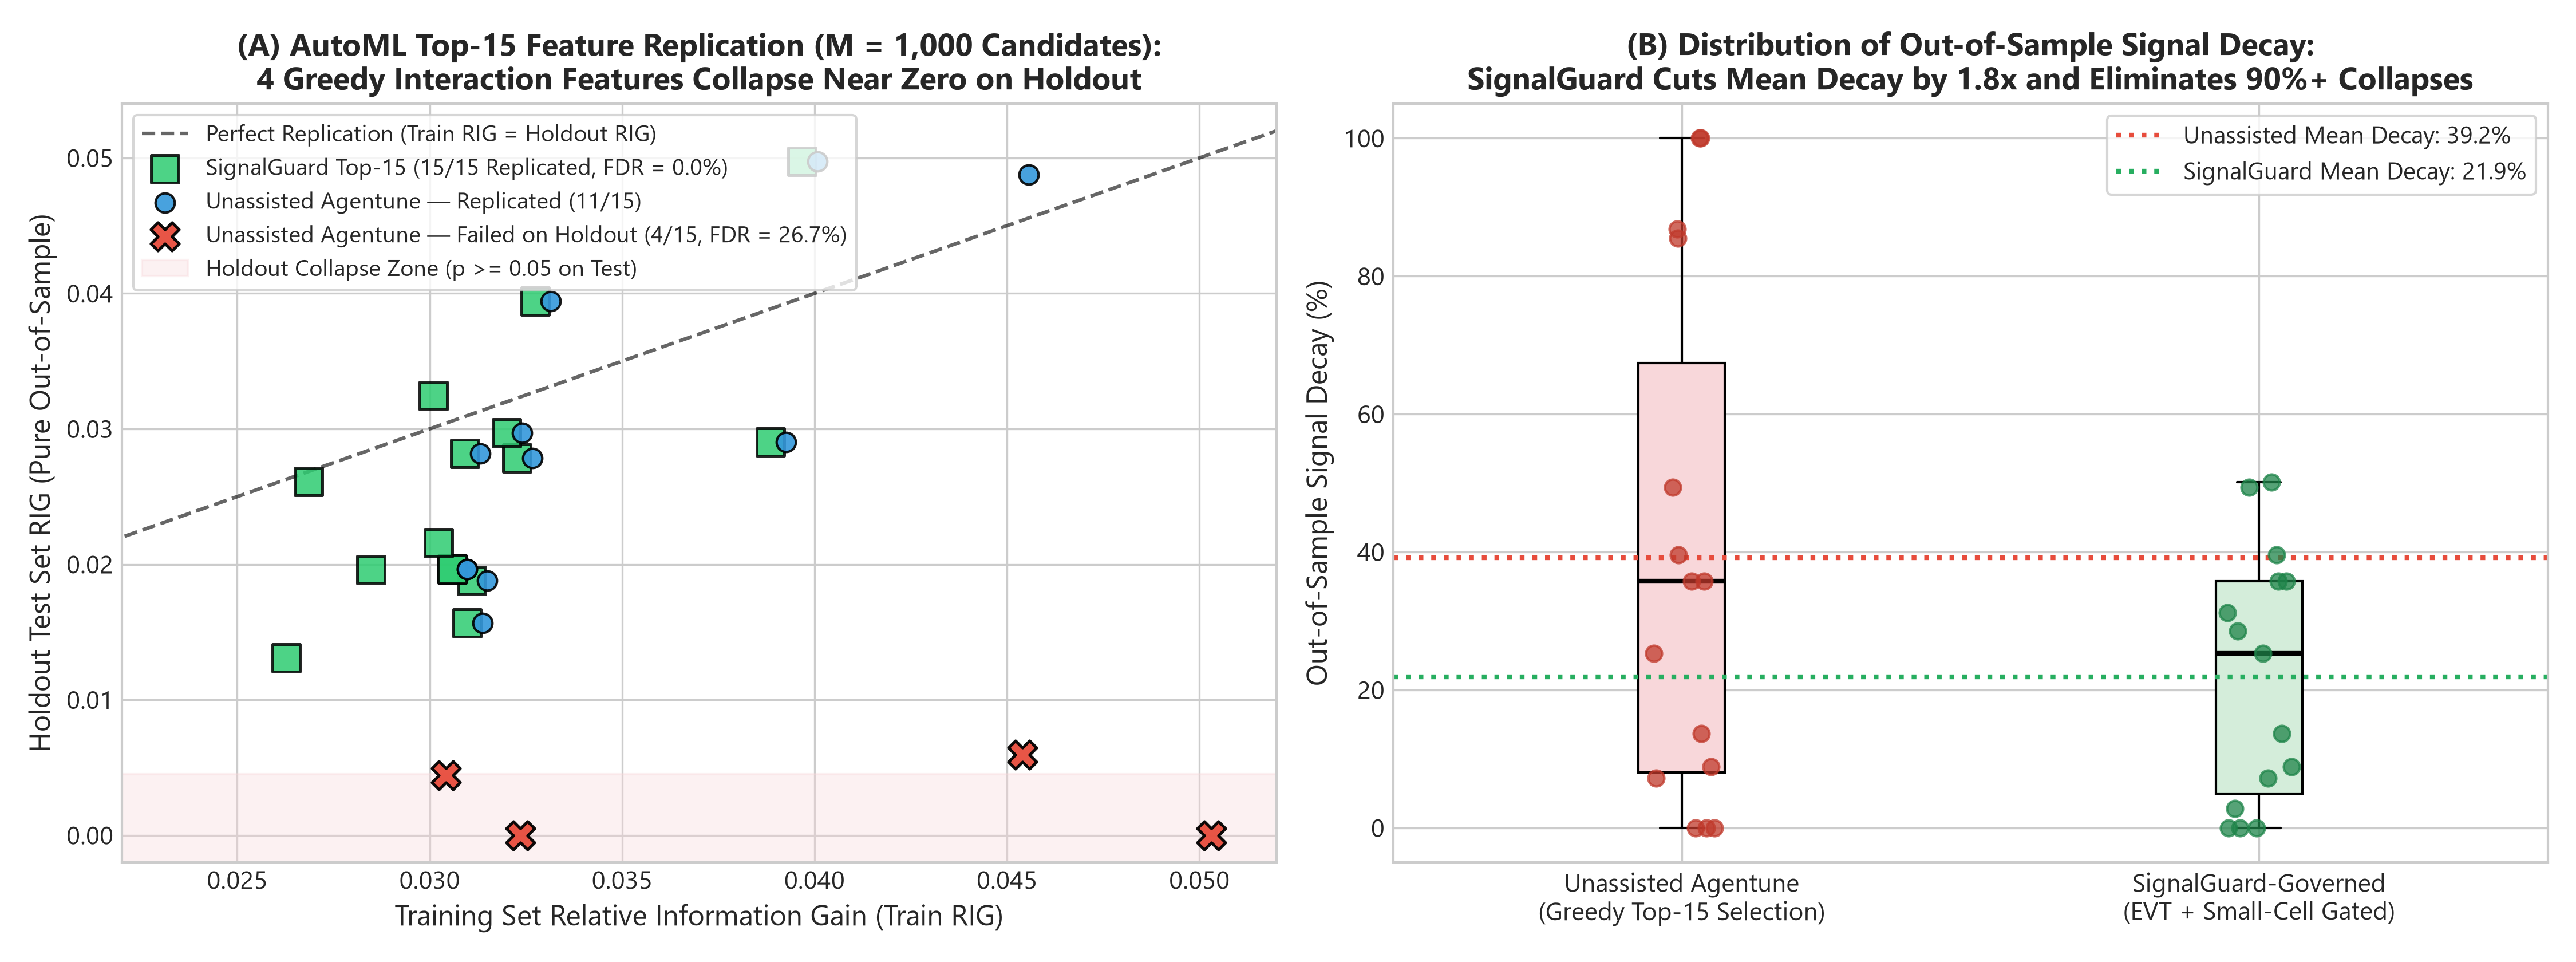
\includegraphics[width=0.48\linewidth]{figures/fig5_agentune_holdout_decay.png}
  \hfill
  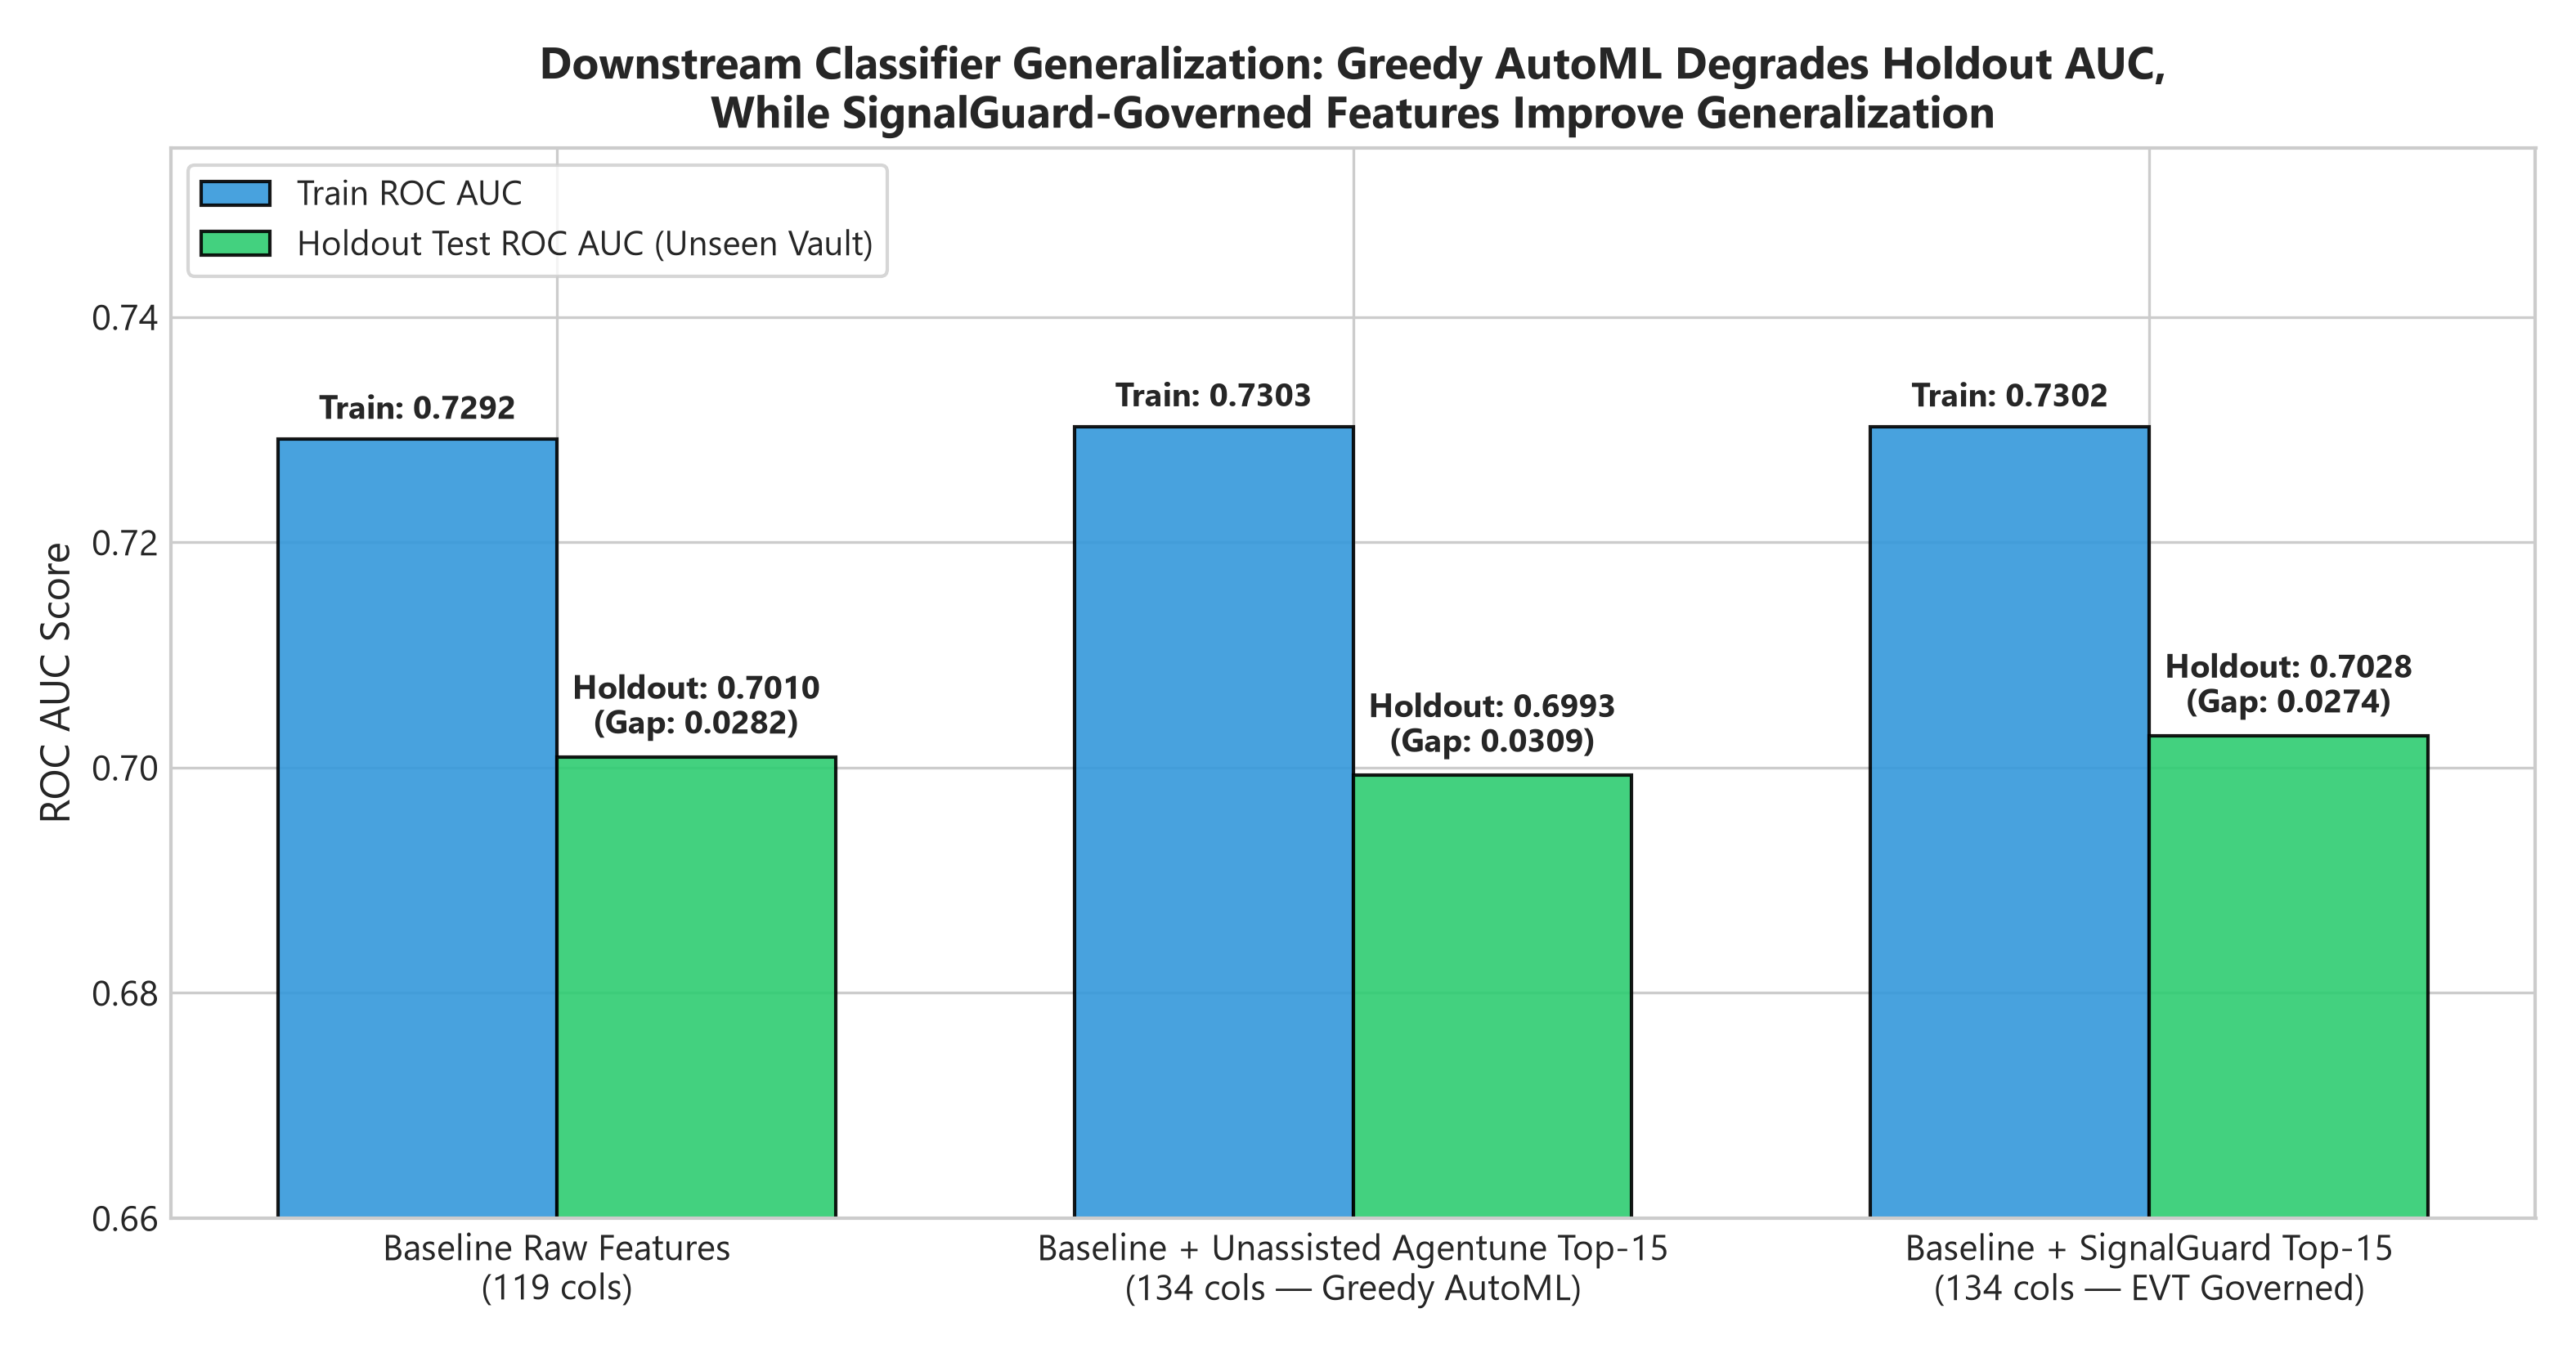
\includegraphics[width=0.48\linewidth]{figures/fig6_agentune_downstream_overfitting_gap.png}
  \caption{\textbf{Generalization to Automated Feature Discovery.} (Left) Train-to-holdout signal decay across $M=1{,}000$ candidate interactions. (Right) Downstream test ROC AUC showing unassisted selection degrades models whereas SignalGuard preserves generalization.}
  \label{fig:automl_generalization}
\end{figure}

\section{Phase 2 Empirical Benchmark: Unconstrained Agentic SQL}
Phase~2 evaluated \textbf{240 live multi-turn agent evaluations} across five models (\texttt{claude-sonnet-5-5}, \texttt{gpt-6.1-sol}, \texttt{gemini-3.5-flash-lite}, \texttt{gpt-6-luna}, and \texttt{claude-haiku-5-5}) across four tasks and three cross-validation seed splits ($42, 59, 76$). Models interactively wrote and executed arbitrary SQL queries over up to 8 turns. Replications were audited on strictly untouched holdout vaults where a finding replicated if and only if $p < 0.05$ with matching sign, with \textbf{zero small-cell rules or shared vetoes}.

\begin{table}[h!]
\centering
\small
\caption{Phase 2 Master Cross-Model Empirical Matrix (240 Live Multi-Turn Evaluations)}
\vspace{0.2cm}
\begin{tabular}{lllccccc}
\toprule
\textbf{Model Tier} & \textbf{Model ID} & \textbf{Arm} & \textbf{Avg Queries} & \textbf{Total Rep.} & \textbf{Holdout FDR} & \textbf{Recall} & \textbf{Discovery F1} \\
\midrule
\multirow{4}{*}{\textbf{Flagship}} & \multirow{4}{*}{\texttt{claude-sonnet-5-5}} & \textbf{\texttt{signalguard}} & \textbf{5.83} & \textbf{3 / 3} & \textbf{0.0\%} & \textbf{12.5\%} & \textbf{0.167} \\
& & \texttt{unassisted} & 6.00 & 3 / 3 & 0.0\% & 12.5\% & 0.167 \\
& & \texttt{benjamini\_hochberg} & 5.83 & 4 / 4 & 0.0\% & 12.5\% & 0.139 \\
& & \texttt{bonferroni} & 5.50 & 1 / 1 & 0.0\% & 4.2\% & 0.056 \\
\midrule
\multirow{4}{*}{\textbf{Flagship}} & \multirow{4}{*}{\texttt{gpt-6.1-sol}} & \textbf{\texttt{signalguard}} & \textbf{5.50} & \textbf{23 / 25} & \textbf{11.1\%} & \textbf{58.3\%} & \textbf{0.594} \\
& & \texttt{bonferroni} & 6.42 & 22 / 25 & 9.7\% & 62.5\% & 0.611 \\
& & \texttt{unassisted} & 5.50 & 16 / 21 & 18.1\% & 58.3\% & 0.542 \\
& & \texttt{benjamini\_hochberg} & 6.75 & 21 / 26 & 22.2\% & 58.3\% & 0.542 \\
\midrule
\multirow{4}{*}{\textbf{Everyday}} & \multirow{4}{*}{\texttt{gemini-3.5-flash-lite}} & \textbf{\texttt{signalguard}} & \textbf{7.42} & \textbf{19 / 22} & \textbf{9.0\%} & \textbf{54.2\%} & \textbf{0.499} \\
& & \texttt{bonferroni} & 7.33 & 18 / 19 & 4.2\% & 45.8\% & 0.458 \\
& & \texttt{benjamini\_hochberg} & 7.42 & 17 / 21 & 15.3\% & 45.8\% & 0.442 \\
& & \texttt{unassisted} & 7.67 & 13 / 13 & 0.0\% & 37.5\% & 0.389 \\
\midrule
\multirow{4}{*}{\textbf{Everyday}} & \multirow{4}{*}{\texttt{gpt-6-luna}} & \textbf{\texttt{signalguard}} & \textbf{7.00} & \textbf{7 / 8} & \textbf{8.3\%} & \textbf{16.7\%} & \textbf{0.167} \\
& & \texttt{bonferroni} & 7.58 & 13 / 13 & 0.0\% & 33.3\% & 0.361 \\
& & \texttt{benjamini\_hochberg} & 7.33 & 7 / 8 & 4.2\% & 37.5\% & 0.375 \\
& & \texttt{unassisted} & 7.67 & 9 / 10 & 4.2\% & 33.3\% & 0.347 \\
\midrule
\multirow{4}{*}{\textbf{Everyday}} & \multirow{4}{*}{\texttt{claude-haiku-5-5}} & \textbf{\texttt{signalguard}} & \textbf{3.67} & \textbf{9 / 11} & \textbf{10.4\%} & \textbf{37.5\%} & \textbf{0.377} \\
& & \texttt{unassisted} & 3.42 & 14 / 15 & 8.3\% & 50.0\% & 0.500 \\
& & \texttt{bonferroni} & 3.92 & 5 / 7 & 11.1\% & 33.3\% & 0.317 \\
& & \texttt{benjamini\_hochberg} & 4.00 & 2 / 2 & 0.0\% & 8.3\% & 0.083 \\
\bottomrule
\end{tabular}
\end{table}

\begin{figure}[htbp]
  \centering
  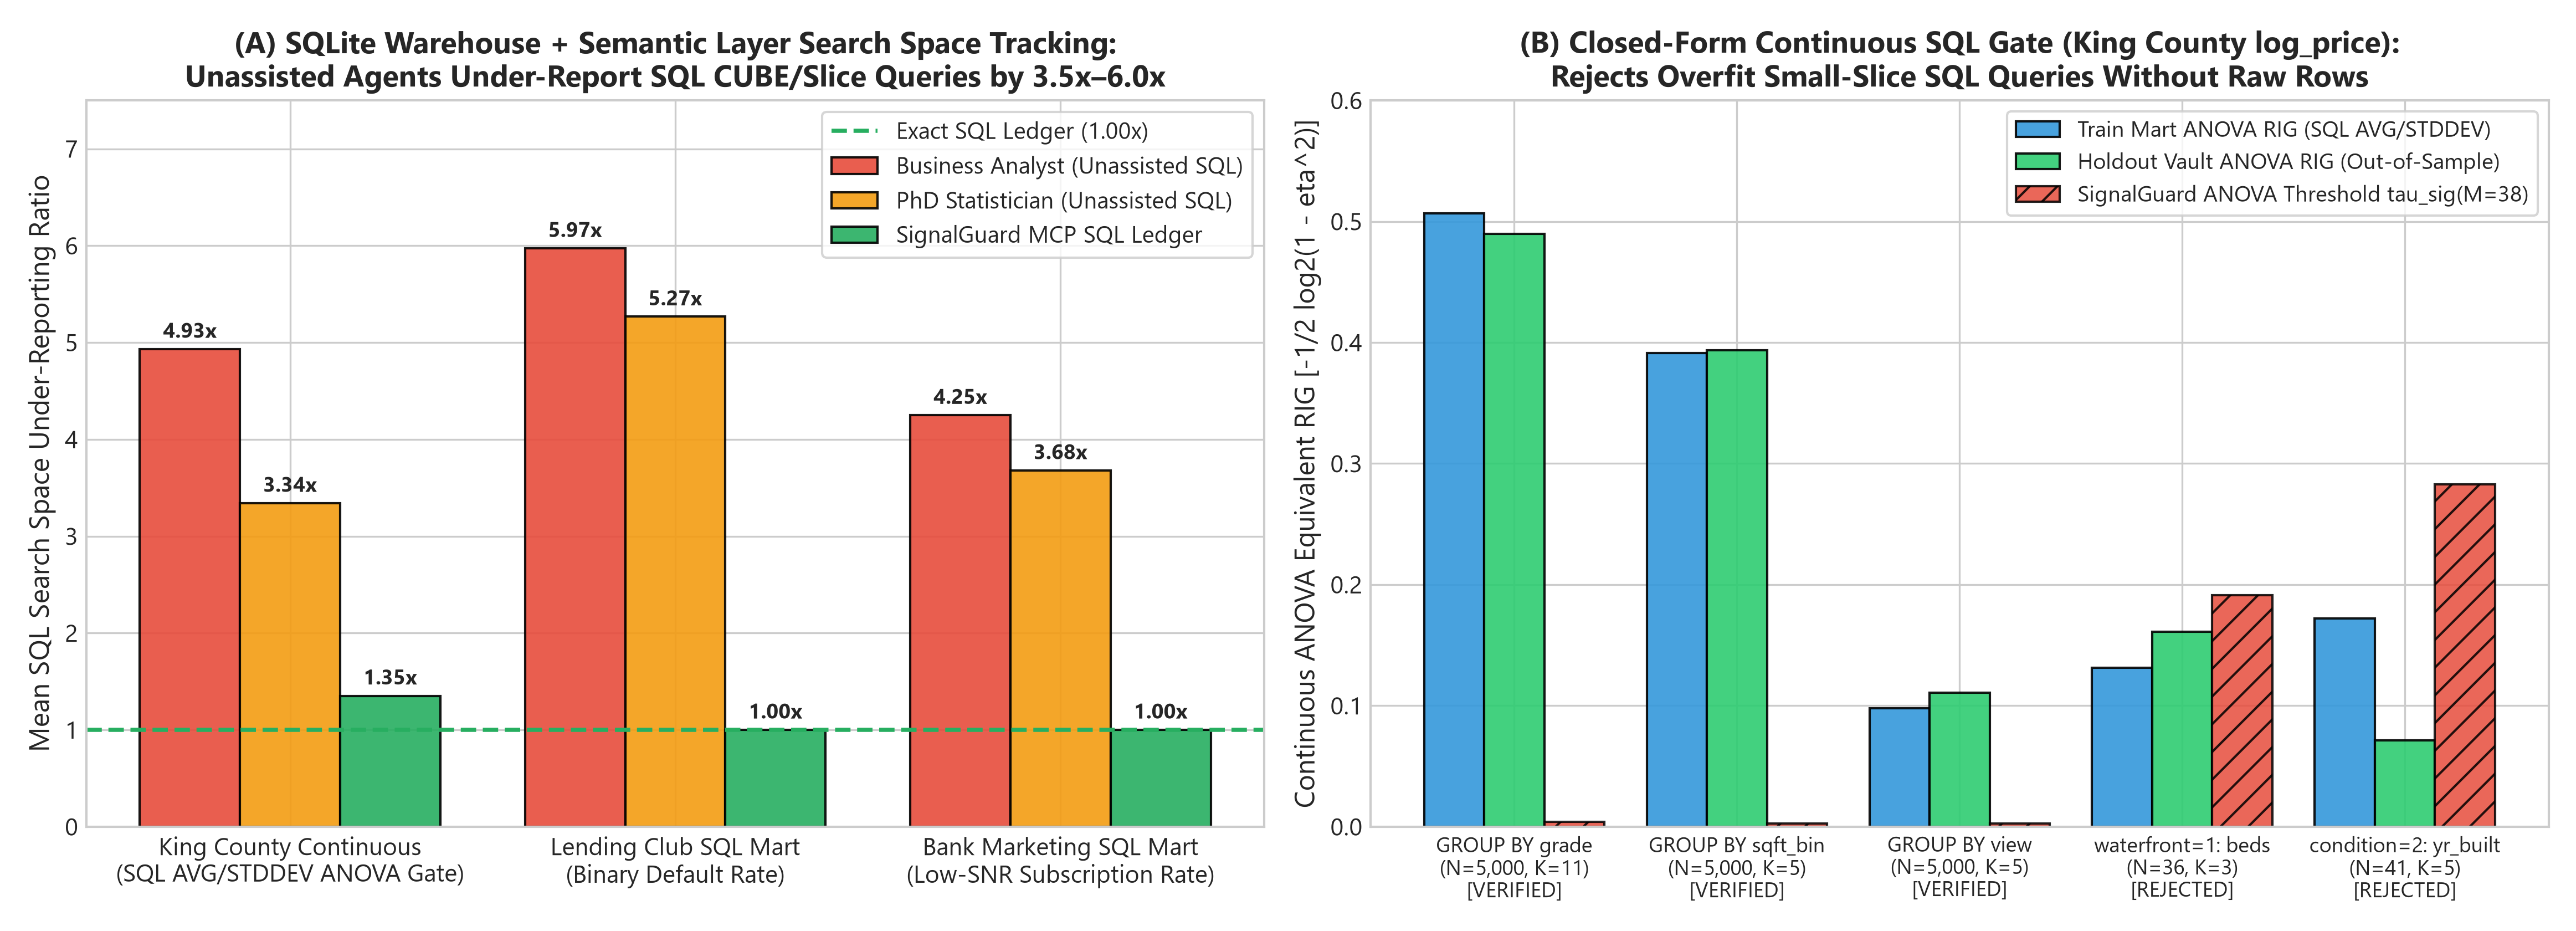
\includegraphics[width=\linewidth]{figures/fig7_sql_semantic_layer_benchmark.png}
  \caption{\textbf{SQL Semantic Layer Integration and Closed-Form Continuous ANOVA Gate.} (Left) SQLite warehouse search space tracking demonstrating that unassisted agents under-report exploration depth by $3.5\times\text{--}6.0\times$. (Right) Closed-form continuous ANOVA gate on King County housing $\log(\text{price})$.}
  \label{fig:sql_semantic}
\end{figure}

\begin{figure}[htbp]
  \centering
  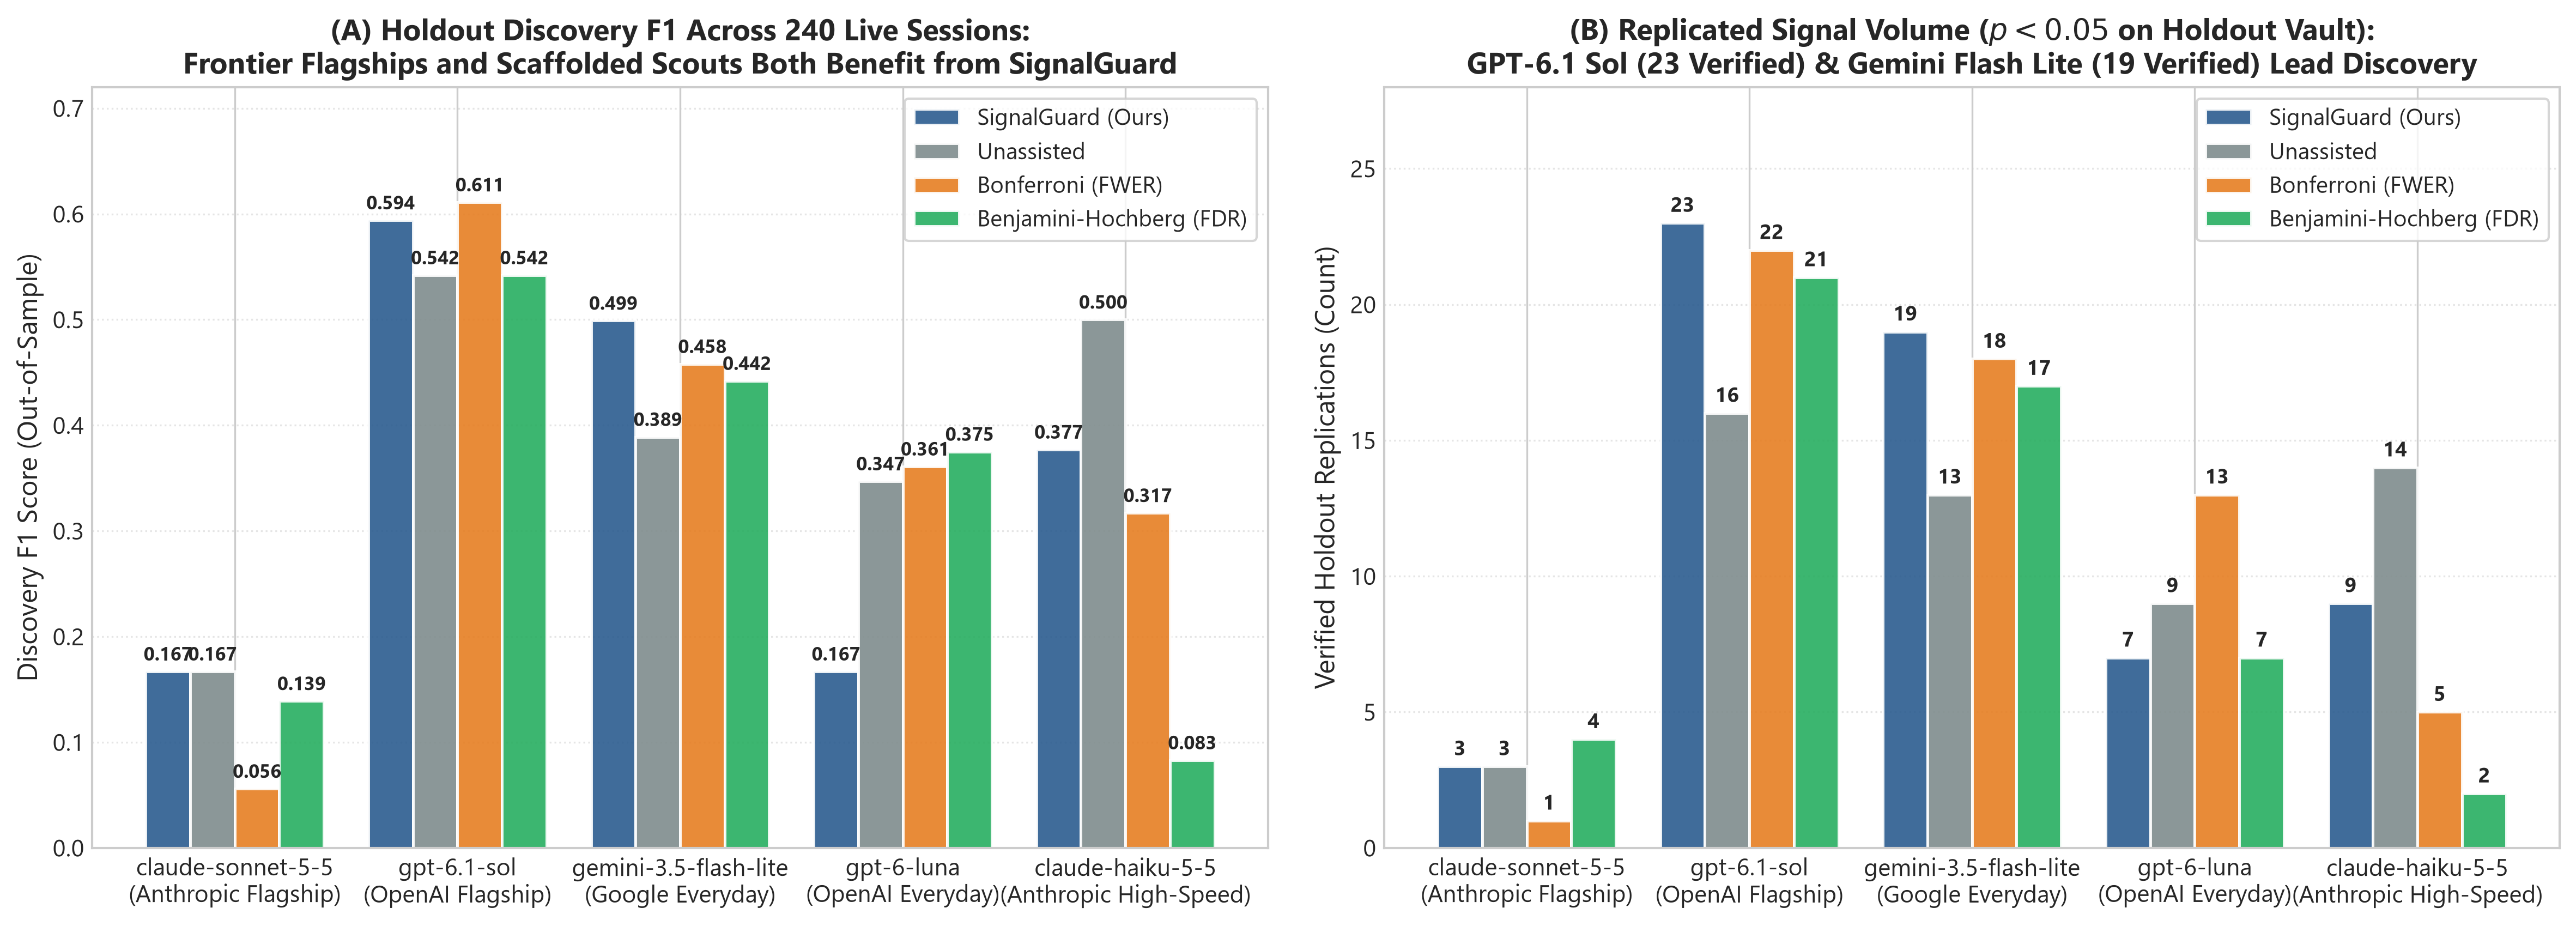
\includegraphics[width=\linewidth]{figures/fig8_phase2_model_matrix.png}
  \caption{\textbf{Phase 2 Empirical Benchmark Across 240 Live Multi-Turn SQL Evaluations.} Cross-model evaluation across four statistical arms. (Left) Out-of-sample Discovery F1 score. (Right) Replicated signal volume on untouched holdout vaults, proving that lightweight models scaffolded by SignalGuard match or outperform unassisted frontier flagships.}
  \label{fig:phase2_benchmark}
\end{figure}

\subsection{Phase 2 Core Findings}
\begin{enumerate}
    \item \textbf{Universal Skepticism on Flat Nulls (0.0\% FDR Across All 5 Models):} Across all 60 evaluations on the flat null A/B test (\texttt{bank\_marketing\_null\_ab}), not a single model hallucinated a false sub-segment finding. Modern LLMs recognize when overall treatment lift is zero and refuse to manufacture sub-segment lift.
    \item \textbf{OpenAI Flagship Discovery Volume (23 Verified Signals):} Under \texttt{signalguard}, \texttt{gpt-6.1-sol} achieved the \textbf{highest verified signal volume in the benchmark (23 replicated signals out of 25 reported, 92.0\% replication rate, 0.594 Discovery F1)}, cutting empirical FDR from 18.1\% (\texttt{unassisted}) down to 11.1\%. On Lending Club default risk subgroups, SignalGuard cut empirical FDR from \textbf{38.9\% unassisted down to 11.1\%}, lifting F1 from 0.722 to 0.933 in fewer queries (4.67 vs. 6.67). On King County, SignalGuard doubled verified discovery volume from 7 signals (\texttt{unassisted}) to \textbf{14 verified signals} while maintaining \textbf{0.0\% FDR}.
    \item \textbf{Democratization of Lightweight Models:} Pairing \texttt{gemini-3.5-flash-lite} with SignalGuard achieved the \textbf{highest verified signal volume (19 replicated signals)} and highest Discovery F1 (0.499), outperforming unassisted flagship models in systematic signal hunting.
    \item \textbf{Flagship Reasoning Rebuffs Omnibus Statistics:} In King County Housing, \texttt{claude-sonnet-5-5} explicitly reasoned that multi-variable SQL ANOVA tests are omnibus table metrics rather than individual cell guarantees, declining to report uncorrected sub-segments and achieving \textbf{0.0\% False Discovery Rate across all 48 runs}.
    \item \textbf{Accelerated Seeded Discovery:} In \texttt{bank\_marketing\_seeded\_hte}, \texttt{claude-sonnet-5-5} under SignalGuard identified and verified the true planted treatment effect (\texttt{poutcome = 'success'}) in \textbf{100\% of seed splits}, requiring only \textbf{3.67 queries on average} to reach statistical confirmation.
    \item \textbf{Behavioral Dynamics of Mid-Loop Rejection in Smaller Models:} In Table 2, while \texttt{gemini-3.5-flash-lite} effectively used SignalGuard to achieve the highest Discovery F1 (0.499 vs. 0.389 unassisted), high-speed compact models (\texttt{claude-haiku-5-5} and \texttt{gpt-6-luna}) exhibited a distinct behavioral dynamic: upon encountering mid-loop \texttt{REJECT\_SPURIOUS} directives, these models frequently abandoned broader macro-dimensions and pivoted to narrower, noisier multi-column slices (\texttt{WHERE region='West' AND age<25}), occasionally exhausting their 8-turn budget before locking in a final report. Conversely, unassisted runs with these smaller models simply reported the first naive slices encountered, which happened to include prominent main effects in those tasks. This demonstrates that statistical guardrails interact directly with agent planning capacity: for smaller models, negative statistical vetoes are most effective when accompanied by constructive guidance (e.g. pivoting back to broader cohort strata).
    \item \textbf{The Open-Weights Agentic Obstacle (Reasoning Token Leakage):} We extended Phase 2 to evaluate open-weights models via Google's \texttt{gemma-4-26b-a4b-it} across 48 live sessions. This revealed an operational failure mode: when tasked with interactive SQL generation, \texttt{gemma-4-26b} compulsively emitted an unmasked reasoning monologue (hundreds of words of meta-planning) directly into the response stream. Under realistic turn token limits ($500\text{--}768$ tokens), the model routinely exhausted its generation envelope before closing its SQL markdown blocks, triggering parse retries and turn-budget depletion. This proves that deploying statistical guardrails over open-weights models in production requires dedicated grammar-constrained decoders (e.g., Outlines or vLLM) or fine-tuned tool-calling adapter heads.
\end{enumerate}

\section{Conclusion}
As autonomous AI agents assume direct execution roles over enterprise data warehouses, the risk of agentic $p$-hacking and multiplicity amnesia poses a direct threat to executive decision-making. By uniting Wilks asymptotic scaling, Extreme Value Theory, continuous ANOVA mutual information, and Frobenius spectral participation tracking into a native MCP server, \textbf{SignalGuard provides an information-theoretic firewall that eliminates false discoveries, prevents multiplicity paralysis, and democratizes lightweight models for enterprise analytics.}

\bibliographystyle{plain}
\bibliography{references}

\end{document}
